\section{Metodi di tracking basati su modelli} \label{modelTracking}
Il \textit{video tracking} è il processo secondo il quale si localizza un oggetto in movimento all'interno di uno stram video e rappresenta uno dei più interessanti problemi di \textit{computer vision}. Esistono svariati approcci al video tracking, ognuno orientato ad ottimizzare le prestazioni relativamente al campo d'azione. In questo lavoro è stata effettuata la scelta di effettuare il tracking secondo l'approccio basato su modelli, che viene eseguito secondo due passi fondamentali: la localizzazione dell'oggetto da tracciare ed il tracciamento effettivo.

Il primo passo, computazionalmente non molto oneroso, è stato realizzato tramite il \textit{background subtraction} (descritto nella sezione ???) e consiste nella rilevazione dell'oggetto all'interno dell'immagine e nell'ottenimento delle informazioni relative.

Il secondo passo, ovvero l'applicazione del tracking al video, rappresenta il punto di maggior interesse del lavoro in quanto consiste nell'elaborazione di una stima della posizione al frame successivo dell'oggetto selezionato; l'esecuzione si basa sull'elaborazione dei dati ottenuti dal processo di localizzazione dell'oggetto.

Gli obiettivi di questo elaborato sono la realizzazione, l'analisi e la comparazione dei due più importanti algoritmi di tracking basato su modelli: il filtro di Kalman, descritto nella sezione \ref{kalman} ed il Condensation, descritto nella sezione \ref{condensation}.

\textbf{Questa parte va espansa mettendo un po' di discorsi sul tracking generale e poi andando a parare sul tracking model based}

\subsection{Kalman Filter}\label{kalman}
Il Kalman Filter\cite{kalman-intro} è un efficiente filtro ricorsivo che valuta e stima lo stato di un sistema dinamico sulla base di una serie di misure soggette a rumore. Il filtro è molto potente in quanto supporta la stima degli stati passati, presenti e futuri del sistema anche quando la natura del sistema è sconosciuta. \'E usato in molti campi ingegneristici, che vanno dall'applicazione in tecnologie radar all'applicazione in computer vision, come utilizzato in questo stesso ambito.
\subsubsection{Definizione del modello}
Il filtro ha l'obiettivo di stimare lo stato $x \in \Re^n$ di un processo a tempo discreto governato dalla seguente equazione alle differenze
\begin{equation}\label{eq:x}
 x_k=Ax_{k-1}+Bu_{k-1}+w_{k-1}
\end{equation} 
dove 
\begin{description}
 \item [$A$] è la matrice di transizione del modello, ed è applicata allo stato precedente $x_{k-1}$; è quindi una matrice quadrata che mette in relazione due vettori delle stesse dimensioni: lo stato al tempo $k-1$ e lo stato al tempo $k$. Risulta la responsabile dell'aggiornamento dello stato.
\item [$B$] è la matrice di controllo sull'input del sistema. \'E applicata al vettore di controllo $u_{k-1} \in \Re^l$ e mappa questo nella dimensione dello stato $x$; è quindi una matrice rettangolare $nxl$.
\item [$w_k \in \Re^n$] è il rumore che affligge il processo. Si assume che sia descritto da una gaussiana a media $0$ e covarianza descritta dalla matrice $Q_k$. Formalmente $w_k \sim N(0,Q_k)$.
\end{description}

Al tempo $k$ l'osservazione dello stato reale $x_k$ è effettuata tramite il vettore della misura $z \in \Re^m$ che è modellato da
\begin{equation}\label{eq:z}
z_k=Hx_k+v_k
\end{equation}
dove 
\begin{description}
 \item [$H$] è la matrice che mappa lo spazio dello stato reale nello spazio dello stato osservato e risulta per questo rettangolare, di dimensione $mxn$.
\item [$v_k \in \Re^m$] è il rumore dell'osservazione, che come per il rumore $w_k$ è descritto da una gaussiana a media zero e covarianza $R_k$. Formalmente si può esprimere come $v_k \sim N(0,R_k)$.
\end{description}
 Da notare che lo stato iniziale ed i vettori che descrivono la presenza di rumore negli stati successivi sono da considerarsi mutualmente indipendenti.

Come detto in precedenza il filtro di Kalman è un estimatore ricorsivo: questo significa che il filtro applica la sua stima dello stato del processo ed ottiene un feedback nella forma del vettore della misura, dal quale può aggiornare la sua computazione. 

Le equazioni del filtro sono raggruppabili in due macrocategorie: \textit{time-update}, responsabili della proiezione nel tempo dello stato corrente per ottenere la stima a prori dello stato successivo (rappresentata dal vettore $\hat{x}_k^- \in \Re^n$), e \textit{measurement-update}, responsabili dell'incorporazione della misura allo stato corrente nella stima a priori, ottenendo così la stima a posteriori (rappresentata dal vettore $\hat{x}_k \in \Re^n$). 

Solitamente lo stadio relativo al \textit{time-update} viene definito come \textit{predict}, mentre quello relatico al \textit{measurement-update} come \textit{correct}.

\begin{figure}[hb]
\centering
	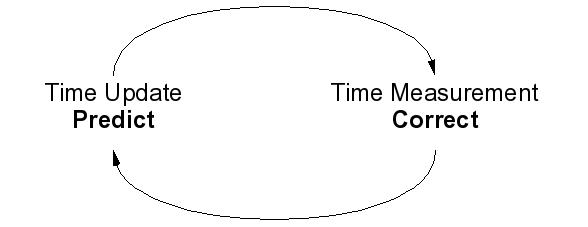
\includegraphics[scale=0.3]{PredCorr.jpg}
\caption{\textit{Il ciclio di calcolo del filtro di Kalman.}\label{fig:predictcorrect}}
\end{figure}
\subsubsection{Predict}
Le equazioni specifiche per il passo di \textit{predict}, che proiettano lo stato e la covarianza dallo stato $k-1$ allo stato $k$ sono 
\begin{equation}\label{eq:prior}
\hat{x}_k^-=A \hat{x}_{k-1}+Bu_{k-1}
\end{equation} 
\begin{equation}
P_k^-=A P_{k-1}A^T+Q
\end{equation} 
dove $A$ e $B$ derivano dalla formula (\ref{eq:x}), considerando sempre la covarianza relativa a $w$ come $Q$, mentre $P_k^-$ è una matrice che rappresenta la covarianza sull'errore nella stima a priori e $P_k$ è una matrice che rappresenta la covarianza sull'errore nella stima a posteriori.
\subsubsection{Correct}

Le equazioni che invece formalizzano il passo di \textit{correct} effettuano una stima sul guadagno del filtro tra l'osservazione attuale e quella predetta (\ref{eq:K}), ottengono la stima a posteriori  (equazione (\ref{eq:post})) data la stima a priori effettuata nel passo di update (\ref{eq:prior}) e dall'osservazione dello stato reale, definita in \ref{eq:z}; viene calcolata anche la covarianza sull'errore nella stima a posteriori (\ref{eq:P}):
\begin{equation}\label{eq:K}
K_k = P_k^- K_T(HP_k^-H^T+R)^{-1}
\end{equation} 

\begin{equation}\label{eq:post}
\hat{x}_k=\hat{x}_k^-+K_k(z_k-H\hat{x}_k^-)
\end{equation} 

\begin{equation}\label{eq:P}
P_k=(1-K_kH)P_k^-
\end{equation} 

\subsubsection{Parametri e configurazione del filtro}
L'esecuzione dell'algoritmo è direttamente dipendente dalla scelta che viene effettuata riguardo ai parametri di configurazione, in particolare dai valori dei componenti delle matrici $Q$ ed $R$.

La matrice che tiene conto della covarianza dell'errore sulla misura, $R$, è generalmente misurata prima dell'applicazione del filtro. Misurare questa grandezza è possibile perchè si suppone di poter misurare il processo in ogni momento, cosicchè possiamo avere anche delle misure ``offline'' con le quali possiamo affinare il calcolo.

La determinazione dei valori della matrice $Q$ invece, è solitamente molto più complicata da ottenere, perchè non c'è la possibilità di osservare direttamente il processo che il filtro sta stimando. 

In entrambi i casi la tecnica solitamente utilizzata per effettuare la stima tramite il filtro di Kalman è di renderlo più performante ``sintonizzando'' i valori di Q ed R e riapplicando il filtro, in modo da determinare empiricamente la miglior configurazione. 

Possiamo notare inoltre che quando nell'esecuzione le matrici $P$ e $Q$ sono costanti, anche la covarianza sull'errore della stima $P_k$ ed il guadagno di Kalman $K_k$ si stabilizzano velocemente fino a rimanere costanti.
\begin{figure}[hb]
\centering
	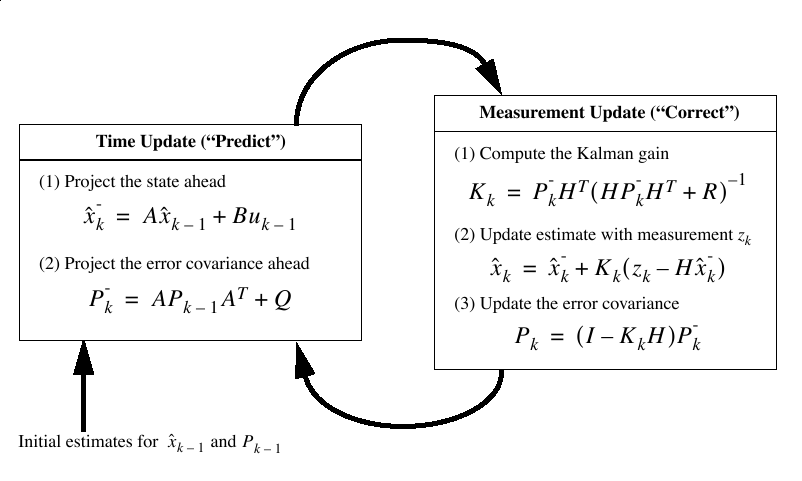
\includegraphics[scale=0.4]{cicloKalman.png}
\caption{\textit{Ciclo di Kalman completo, con parametri ed equazioni}\label{fig:completeKalman}}
\end{figure}

\subsection{ConDensation}\label{condensation}
\cite{condensation}\textbf{descrivere seriamente il particle filter (tipo dagli articoli o dalla wiki) mettendo anche dettagli matematicosi}

\subsection{Descrizione dell' implementazione dei modelli}
Fare cappello su cosa è un modello poi particolareggiare verso il nostro modello

QUESTA PARTE VA FATTA BENE

ricordarsi di mettere la descrizione del background subtraction per quanto riguarda il ruolo dell'oggetto.

come sono fatte le matrici che descrivono 
dire che noi s'ha un generico sistema descritto unicamente dalla sua posizione sul piano e dalla sua velocità orizz e verticale

Cosa si prende per varianza di uno dell'altro, come è fatto lo stato (vettore i 4 dimensioni di cui 2 posizione xy etc..)
